\documentclass[12pt]{article}
\usepackage{times}
\usepackage{plext}
\usepackage{cite}
\usepackage{setspace}
\usepackage{float}
\usepackage{lineno}
\usepackage{color}
\usepackage[dvipdfmx]{graphicx}
\usepackage{array, booktabs}
\usepackage[top=25truemm,bottom=25truemm,left=30truemm,right=30truemm]{geometry}
\usepackage{threeparttable}
\usepackage{ulem}
%\usepackage{amsmath}
\renewcommand{\figurename}{Fig.}
\renewcommand{\tablename}{Table}
\begin{document}\setcounter{page}{1}
\renewcommand\citeleft{(} 
\renewcommand\citeright{)}

\flushleft{\textbf{Title: Integrated species distribution model improves spatial uncertainty of eDNA of Edomae-fish in Tokyo Bay}}\\
%Integrated spatial model estimates the fish distribution using environmental DNA and catch data
%\flushleft{\textbf{Running title: }}\\
\flushleft{Yuki Kanamori$^{1\ast}$, Hiroshi Okamura$^{2}$, Shota Nishijima$^{2}$, Yuki Hongo$^{2}$, Yasuyuki Uto$^{3}$, Hisatoku Mita$^{4}$, Mitsuhiyo Ishii$^{4}$, Kiyoharu Akimoto$^{5}$, and Akane Kusano$^{6}$}\\
\ \\
$^{1}$ Fisheries Resources Institute, Japan Fisheries Research and Education Agency, 25-259 Shimomekurakubo, Samemachi, Hachinohe, Aomori 031-0841, Japan\\
$^{2}$ Fisheries Resources Institute, Japan Fisheries Research and Education Agency, 2-12-4 Fukuura, Kanazawa, Yokohama, Kanagawa 236-8648, Japan\\
$^{3}$ \\
$^{4}$ \\
$^{5}$ \\
$^{6}$ \\
\ \\

$^{\ast}$ Corresponding author\\
Email: kana.yuki@fra.affrc.go.jp

\newpage
\flushleft{\textbf{Abstract}\\}

\flushleft{\textbf{Keywords}}\\
Spatial distribution, Environmental DNA, data fusion, Spatial correlation, Ecology of eDNA

\newpage
\begin{linenumbers}
\setstretch{2}
\section{Introduction}
Understanding of spatial distribution of species and underling its mechanism is a major goal in ecology. 
Field surveys using environmental DNA (eDNA) are widely used for monitoring such as endangered species, invasive species (e.g., Dougherty et al. 2016%ザリガニJ appl ecol
; Larson et al. 2020%レビュー
), and biodiversity 
%detecting invasive or rare species and hotspot of biodiversity %(面倒なのでレビュー論文を引用) 
because the surveys of eDNA are easy to detect occurrence of target species, non-invasiveness, and high cost effectiveness rather than previous direct sampling method (Rees et al. 2014; Thomsen \& Willerslev 2015). %Dorazioに引用されていたやつ.あとで再確認
However, uncertainty of the occurrence of eDNA is a issue in eDNA studies because various factors, such as biological and environmental features, intricately affect the shedding (i.e., production of eDNA from organisms) and degradation (i.e., decay of eDNA from a system) of eDNA (Fig. 1). Therefore, it is necessary to consider the spatial uncertainty included in eDNA to infer the spatial distribution of species from eDNA occurrence data.


%However, a issue of eDNA is uncertainty of the occurrence of eDNA caused by various factors such as biology and environment (Fig. 1). 
%However, the occurrence of eDNA includes many types of uncertainties due to relating to environmental factors such as temperature and advection ().For example, in aquatic habitats, it is not sure whether target species are in a location or not when eDNA of target species is detected because eDNA are transported passively.Therefore, the consideration to the influence of environmental factors on eDNA is necessary for estimation of species distribution when we use eDNA methods.

\ \ \ \ \ \ \ \ \ \ 
After the suggestion of the importance of understanding about origin, state, transport, and fate of eDNA ("ecology of eDNA") by Barnes \& Turner (2016), the studies which used laboratory experiments and numerical hydrological models have been increased to overcome the uncertainty of eDNA. 
%To overcome the uncertainty of eDNA, the studies which used Laboratory experiments and numerical hydrological models have been increased after suggested the importance to understand about origin, state, transport, and fate of eDNA ("ecology of eDNA") by Barnes \& Turner (2016).
%Laboratory experiments and numerical hydrological models have been used to overcome the uncertainty of eDNA, because Barnes \& Turner (2016) suggested the importance of knowledge about origin, state, transport, and fate of eDNA ("ecology of eDNA").  
% Laboratory experiments and numerical hydrological models have been used to overcome the uncertainty of eDNA, especially after suggested the importance of "ecology of eDNA" by Barnes \& Turner (2016).
For example, the relationship between production rate of eDNA and biological factors (e.g., species and body mass) or environmental factors (e.g., temperature), and between decomposition of eDNA and the sate of eDNA (e.g., length of eDNA) or environmental factors were measured. In numerical hydrological models, spatial distribution of eDNA was simulated in aquatic area and obtain the production, transport and decay of eDNA (e.g., Fukaya et al. 2020). %深谷さんの論文に引用あり
However, keeps for all focal species in laboratory are not realistic and low cost-efficiency when multi species studies such as biodiversity monitoring and fisheries management. Moreover, biologists monitoring species are not often familiar with hydrological models and the simulation of eDNA seems to be hard for them.

\ \ \ \ \ \ \ \ \ \ 
Integrated species distribution models (IDMs) are now common spatial model to predict spatial pattern of species (Issac et al. 2020).
% As alternative approach to over come the spatial uncertainty of eDNA, statistical modeling approach should be a useful approach.
%The model use the different type of data with strengths and weaknesses, such as scientific survey data which is restricted spatially and quantitatively and opportunistic citizen data which is widely collected and abundant, and combine in a single model (Isaac et al. 2020; Miller et al. 2019).
%The model use the different type of data with strengths and weaknesses, such as scientific survey data (high quality but not abundant) and opportunistic citizen data (low quality but abundant) , and combine in a single model (Isaac et al. 2020; Miller et al. 2019).
The models combine the different type of data with strengths and weaknesses in a single model. For example, the model can use both scientific survey data, which is high quality but less abundant due to restriction of cost, and citizen data, which is widely collected and abundant but may be low quality due to not using consistent field methods in a model.
%scientific survey data are high quality but less abundant due to restriction of spatially costly while opportunistic data such as citizen data are widely collected and abundant but may be low quality due to not using consistent field methods.
Combining both types of data can capitalize on the strengths of each data and perform better prediction than models when using single data (Pacifici et al. 2017; Miller et al. 2019). 
Hence, if we develop a IDM that uses not only the occurrence data of eDNA but also the second data which contains the information that species exists at a location, as well as environmental factors as covariance in the model, then the inference from the model should represent the reduction of the spatial uncertainty of eDNA and improvement (Fig. 1).
%reduction of the spatial uncertainty of eDNA and improvement of the inference of spatial distribution from eDNA should be expected (Fig. 1).
%the spatial uncertainty of eDNA should be reduced and the model inference should be improved (Fig. 1).
%Hence, if we develop a IDM that uses not only eDNA data but also the second data which contains the information that species exists at a location, then the model inference of the spatial distribution should be reduced about spatial uncertainty of eDNA and should be improved.   
%したがって,統合モデルにより『生物がその場所に生息する』という情報をeDNAに加えることで,eDNA
%したがって,eDNAデータと新たなデータ(『生物がその場所に生息する』という情報を持つ)を使って統合モデルを構築すれば,eDNAデータに対する空間的な不確実性は減少し,eDNAから推定される空間分布の精度は上昇することが期待される.


%\ \ \ \ \ \ \ \ \ \ 
%Tokyo Bay is a large enclosed coastal sea in Japan. There are many commercially important species for fisheries that are called "Edomae" in Tokyo Bay because these species have been used for Sushi since Edo Era (about 400 years ago). Catch weight of some Edomae have been decreased because of habitat modification due to urbanization (e.g., landfill of tidal flats and water pollution). Catch statistics (total catch weight in each species, efforts, and geographic location of fishing) have been collected for stock assessment since \textcolor{red}{1990} by prefectures around Tokyo Bay. The strengths of this data are the direct evidence that a focal species occupies a location of fishing and abundant because of widely collected in Tokyo Bay.  On the other hand, weakness of this data is like a opportunistic data because the data is likely to be biased towards areas to high density of focal species due to commercially fishes, consequently less zero data. In addition to this catch statistics, scientific survey of eDNA has been conducted monthly since 2018 for biodiversity monitoring because biodiversity also may decreased due to human-induced environmental changes in Tokyo Bay (Hongo et al., submitted). The strengths are that the data is systematically collected data and includes zero data, while the weaknesses are that the data is less abundant due to spatial restriction of the survey and includes spatial uncertainty in the occurrence of eDNA as description in above.


\ \ \ \ \ \ \ \ \ \ 
In this paper, to infer spatial distribution of species from the occurrence data of eDNA, we first make a spatial distribution model which considers spatial uncertainty of eDNA by using an integrated spatial distribution model. We then applied the model to both eDNA data and catch weight data for four fish in Tokyo Bay, Japan, and predicted the spatial distribution of these fish. We finally compared the differences in (i) the predicted spatial distribution of eDNA among fish and (ii) the relationship between the occurrence of eDNA and environmental factors among fish to discuss the effects of the biological factors on the spatial uncertainty of eDNA.

%And finally, we compared the differences in the predicted spatial distribution among fish and discuss the relationship between the pattern of the inference of spatial distribution and biological characteristics of fish.

%to predict spatial distribution of species from eDNA, we first make a model which considers uncertainties of eDNA caused by environmental factors without additional laboratory experiments and numerical hydrodynamic models, by using an integrated spatial distribution model (eDNA-IDM). 

%In this paper, we make an integrated spatial distribution model by combining both catch statistics, which is opportunistic data but abundant and represents the direct evidence where fish was, and eDNA data, which is the monitoring data in the same points but not abundant and includes uncertinties due to environmental factors.

%In this paper, we make the model considering with uncertinties caused by environmental factors, such as temperature and advection, to predict spatial distribution of species using an integrated spatial distribution model. 

\ \\

\section{Materials and Methods}
%2.1: a general model to estimate species distribution from eDNA
%2.2: an application to a eDNA and catch data in Tokyo Bay
%2.2.1: 野外調査
%2.2.2: 漁獲量データ
%2.2.3: model in Tokyo Bay


\subsection{A general model to estimate species distribution from eDNA}
\flushleft{\textbf{Features of integrated spatial distribution model}}\\
Integrated spatial distribution model that account for explicitly spatial autocorrelation in occurrence were built by Pacifici et al. (2017), which shows three approaches to predict the spatial distribution of species: the joint likelihood (shared), correlation, and covariate methods. The joint likelihood method uses multiple data types to simultaneously estimate a shared set of parameters with constraining that the likelihoods of shared set of parameters to be equal across. The correlation method connects multiple data types indirectly through a shared covariance matrix that captures similar patterns present in each data sources. The covariate method incorporates information from a added dataset via a fixed effect. 

\ \ \ \ \ \ \ \ \ \ 
Although each methods estimate the spatial distribution of species using multiple data sets, we need to select method depending on the data features for analysis because there are strengths and weaknesses (Pacifici et al. 2017; Miller et al. 2018). The joint likelihood method may be problematic when the second data is of poorly quality compared to correlation and covariate methods because each data can directly inform the latent occurrence state (probabilities?) and the weight given to estimate the parameters is naturally determined by their relative size and quality. Thus, it is not the best method when our second data is low quality while it is the best method when our second data is high quality (vise versa). 
%The joint likelihood method simultaneously fits a likelihood to both data sources
%The joint likelihood approach uses multiple data types to simultaneously estimate a shared set of parameters.
%the shared set of parameters within each of the individual likelihoods is constrained to be equal across likelihoods.
The correlation method is added robustness to the joint likelihood because the second data indirectly inform the occurrence state. Thus, it is the best method when our second data is low quality while it is inferior to the joint likelihood method when both data are deemed reliable.
%The correlation method is added robustness to the joint likelihood for the influence of unreliable data because the second data indirectly inform the occurrence state.
% while this method is inferior to the joint likelihood when both data are deemed reliable.  
The covariate method does not make full use of the information in the second data because the second data as a constructed covariate in the mean occurrence state. In addition, this method can reduce the computational cost because there are fewer parameters to estimate and the number of data locations can be reduced. Thus, it is the best method when the second data is low quality and/or there is computational limitation while it may not the best method when the information of the second data is needed.


%\ \ \ \ \ \ \ \ \ \ 
%As described above, 
%When predicting the spatial distribution of species from eDNA, eDNA data is often collected systematic method (e.g., collected at the same sites and efforts)

%When predicting the spatial distribution of species from eDNA using integrated species distribution model, the information that a species exists as second data is needed because of spatial uncertainties of eDNA due to complex factors. 
\flushleft{\textbf{The model for eDNA}}\\
When predicting the spatial distribution of species from eDNA using integrated species distribution model, the information that a species exists is needed as second data to consider spatial uncertainties of eDNA due to complex factors (Fig. 1). Hence, the second data is preferred to high quality as possible. 
%However, spatially widely collected data and/or 
%しかし,空間的に広く,また調査データのように系統的に取得されているデータを2番目のデータとして使用できるケースは限られているかもしれない.なぜなら,eDNAは直接的なモニタリングに比べて簡易的であるためより広い範囲で取得されており,またコンタミを防ぐためにも厳密な調査手法によって取得されている可能性が高いからである.
%したがって,2番目のデータがhigh qualityであることは期待できないかもしれない.

しかし,eDNAは直接的なモニタリングに比べて簡易的であるためより広い範囲で取得されている可能性が高く,eDNAのデータと同様の空間範囲で調査データのように質の高いデータを取得することは難しいかもしれない.その一方で,eDNAの空間的な不確実性を考慮するためには,種がいた証拠である2番目のデータの情報をeDNAのデータにしっかりと伝える必要がある.これらを考えると,integrated spetial distribution modelを用いたeDNAからの空間分布の推定には,以下のようなcorrelation methodが適切である: 

\begin{equation}
\begin{array}{ll}
p_{e}(s_{i}) = \alpha_{e} + \sum_{k}f_{e, k}(x_{e, k}(s_{i})) + w \theta(s_{i}) + u_{e}(s_{i})\\
p_{a}(s_{i}) = \alpha_{a} + \sum_{k}f_{a, k}(x_{a, k}(s_{i})) + \theta(s_{i}) + u_{a}(s_{i})\\
%\]
%\[
%\]
\end{array}
\end{equation}
where $\alpha$ and $x_{k}(s_{i})$ are the intercept and the covariates at sites $i$ for occurrence probabilities at sites $i$ of the added data ($p_{a}$) and eDNA data ($p_{e}$), respectively. $u(s_{i})$ is spatial error that is specific for each data following multivariate normal distributions $\mathrm{MVN}(0, \mathbf{R})$, where the variance--covariance matrix $\mathbf{R}$ is a Mat\'{e}rn correlation function. $\theta$ which is shared between two equations is the common spatial pattern between the two data, which cannot explain by each terms of the equations. That is, $\theta$ can be interpreted as "true" spatial distribution of species.





%\[
%\mathrm{logit}(p_{1}(s_{i})) = \alpha_{1} + \beta(s_{i}) + \theta(s_{i}) + u_{1}(s_{i})
%\]
%\[
%\mathrm{logit}(p_{2}(s_{i})) = \alpha_{2} + \sum_{k}f_{k}(x_{k}(s_{i})) + w \theta(s_{i}) + u_{2}(s_{i})
%\]



\subsection{An application to a eDNA and catch data in Tokyo Bay}
\flushleft{\textbf{2.2.1 eDNA data}}\\
\flushleft{\textbf{Field surveys}}\\
Field surveys were conducted by prefectural experimental station in Chiba, following the consistent sampling design at 14 sites in Tokyo Bay from April to December in 2018 (Fig. 1). 
%Field surveys were conducted at 14 sites in Tokyo Bay from April to December in 2018 using R/V Fusanami or R/V Fusami-maru of Chiba Prefecture and R/V Enoshima-maru of Kanagawa Prefecture (Fig. 1). 
In each sites, seawater and environmental data were simultaneously collected. For eDNA analysis, two litter of bottom seawater was collected using a Niskin water sampler, and then it was separated for two 1L samples for replicate. Each samples filtered glass fiber membrane GF/F (0.7 $\mu m$ pore size; Cytiva, Sheffield, UK) onboard and then the filters were frozen on a block of dry ice. These frozen filters were stored at $-30^\circ$ in the laboratory until eDNA extraction. To lower the levels of cross-contamination, equipments for eDNA sampling were changed new one or washed in each sites. During sampling the bottom seawater, seawater temperature, salinity, pH, and dissolved oxygen (DO) at the same depth of seawater sampling for eDNA were measured by CTD (メーカー).
%The egg surveys were conducted by 18 prefectural experimental stations or fisheries research institutes and two national research institutes of the Japan Fisheries Research and Education Agency, following the consistent sampling designs, as a part of the stock assessment project.

\flushleft{\textbf{Laboratory experiments}}\\
In laboratory, eDNA extraction, eDNA amplification, and eDNA sequence were conducted. Total eDNA was extracted from the frozen filters using a DNeasy Blood and Tissue Kit (Qiagen, Hilden, Germany) following Yamamoto et al. 2019. Mitochondorial 12S rRNA gene was amplified using MiFish universal primers referring to Miya et al. 2015 with slight modification. The details was shown in Hongo et al. (受理されてないようだったら書くしかない).  eDNA sequence were ....


\flushleft{\textbf{2.2.2 Catch statistics}}\\
A part of catch statistics of small-scale bottom trawl fisheries recorded by several representative boats of Chiba Prefecture were provided by Chiba Prefecture. This data included date, geographic location, efforts (number of tows), gear, and catch weight (kg) in each fish. Almost of all gear was beam trawl although dredge net also used. The species which also detected by eDNA was \textit{Conger myriaster} (マアナゴ), \textit{Kareius bicoloratus} (イシガレイ), \textit{Lateolabrax japonicus} (スズキ), and \textit{Konosirus punctatus} (コノシロ). Thus, we estimated the spatial distribution of these four species using the eDNA-IDM. \textcolor{red}{マコガレイ,カマス類,クロダイ,イシモチ類も解析できる??}

\flushleft{\textbf{2.2.3 Estimation of spatial distribution}}\\
To estimate the spatial distribution of four focal species using eDNA and catch data by considering with spatial  uncertainties of eDNA, we fitted the model (equation 1) to the presence/absence of eDNA and of catch collected in Tokyo Bay as follows:
%In this study, to estimate the spatial distribution of species from eDNA considering with spatial uncertainties, we make a integrated species distribution model using correlation method.
\[
\mathrm{logit} \ \ p_{e}(s_{i}) = \alpha_{e} + \sum_{k}f_{k}(x_{k}(s_{i})) + w \theta(s_{i}) + u_{e}(s_{i})
\]
\[
\mathrm{logit} \ \ p_{c}(s_{i}) = \alpha_{c} + \beta_{i} + \theta(s_{i}) + u_{c}(s_{i})
\]
where $\alpha$ is the intercept, and $x_{k}(s_{i})$ is the covariates at sites $i$ for occurrence probabilities of eDNA at sites $i$. In the study, seawater temperature, salinity, pH, and DO were used as covariates which effect on the occurrence of eDNA (i.e., $k = 4$). $u(s_{i})$ is spatial error that is specific for each data following multivariate normal distributions $\mathrm{MVN}(0, \mathbf{R})$, where the variance--covariance matrix $\mathbf{R}$ is a Mat\'{e}rn correlation function. $\theta$ which is shared between eDNA and catch is the common spatial pattern between the two data, which cannot explain by each terms of the equations. That is, $\theta$ can be interpreted as the spatial distribution of species we want to know. \textcolor{red}{共変量の非線形性について書く}Parameters in this model was estimated by Integrated Nested Laplace Approximation using using the R-INLA package (Lindgren, 2012) in \textcolor{red}{R 3.6.1 (R Development Core Team, 2019).}
\ \ \ \ \ \ \ \ \ \ 




\ \\
%\setstretch{1}
\flushleft{\textbf{\Large{Acknowledgments}}}\\
This research was financially supported by Grant-in-Aid for Fisheries Agency of Japan.
%This research was financially supported by the grants from the Japan Society for the Promotion of Science (JSPS) (19K15905, 20392904).
\ \\

\flushleft{\textbf{\Large{Authorship}}}\\
YK conceived of the research idea. YH, YU, HM, MI, KA, and AK conducted field sampling. YH performed the laboratory experiments. YK, HO, and SN designed statistical analyses. YK wrote programs and performed the analyses. YK wrote the manuscript with input from all co-authors' comments.
\ \\

\newpage
\begin{figure}[h]
  \centering
  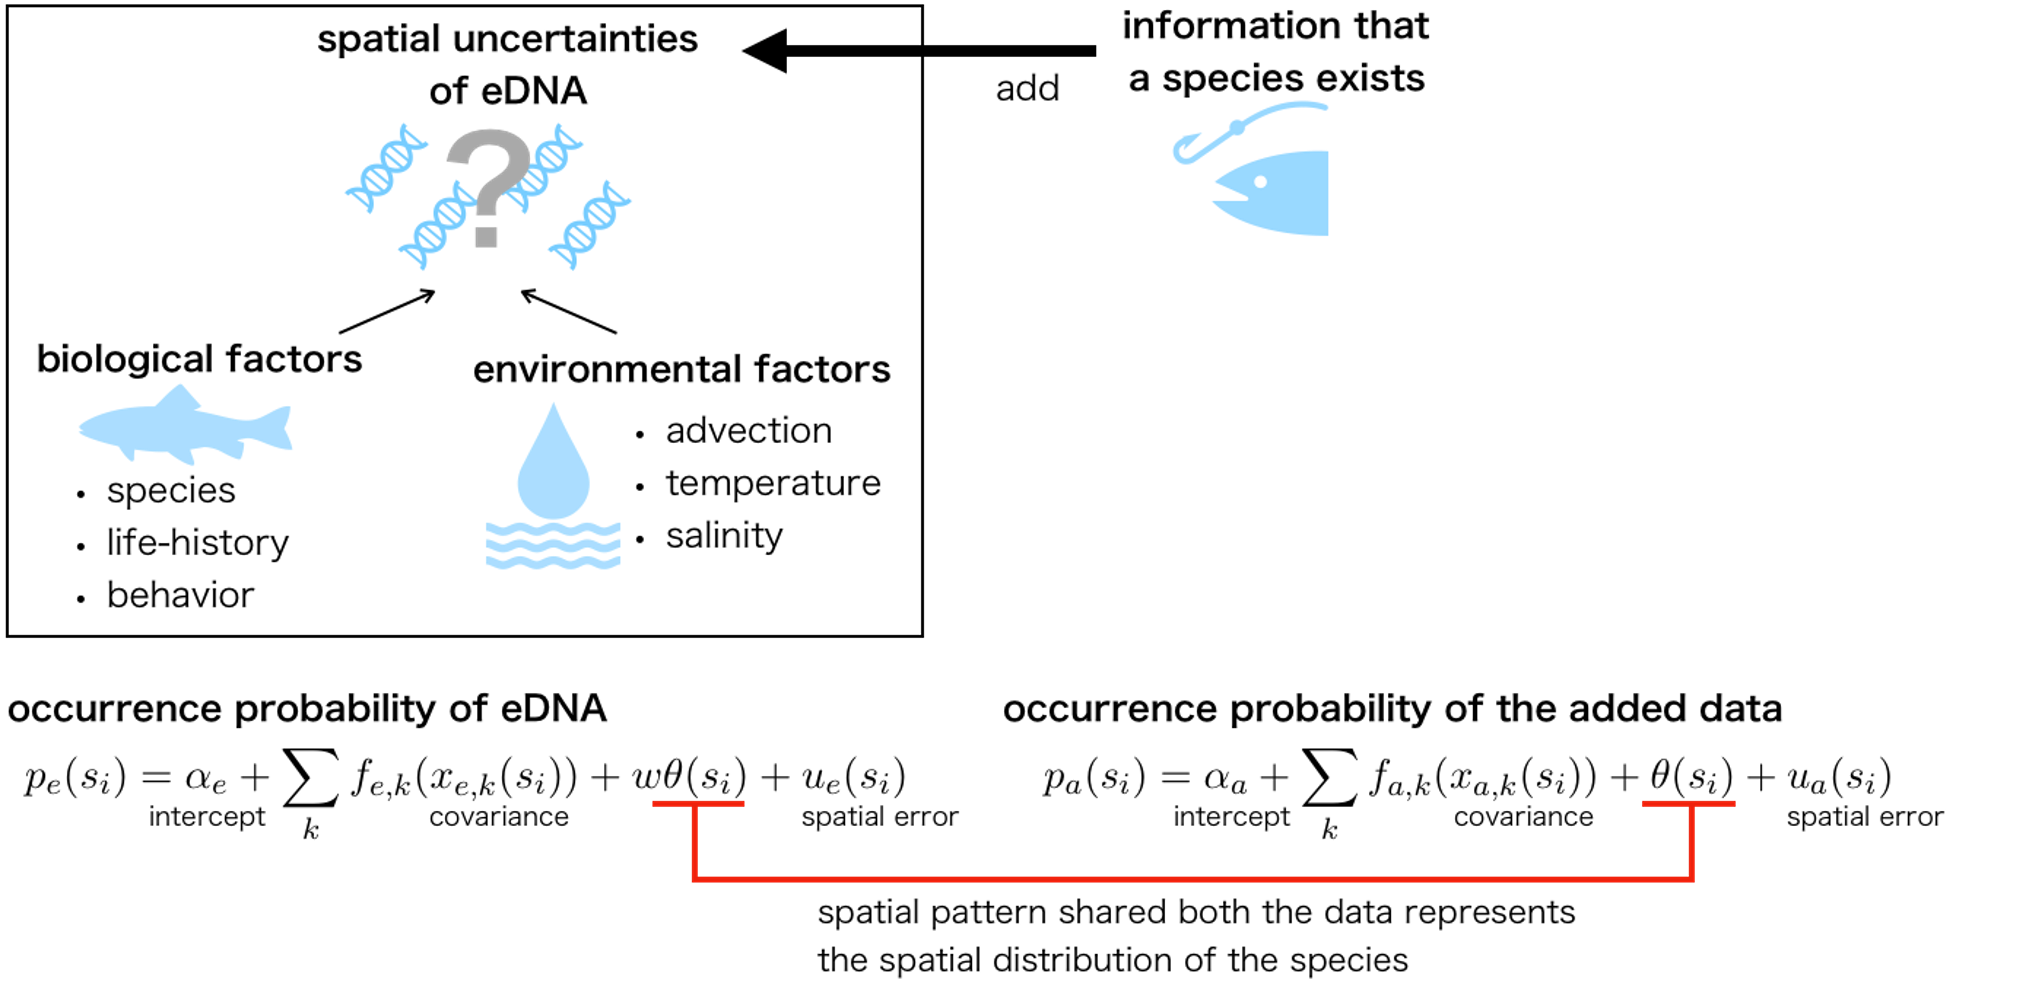
\includegraphics[width = 18cm]{fig1.png}
  \caption{Conceptual diagram of this study.}
\end{figure}



\end{linenumbers}
\end{document}
